\documentclass[hyperref, a4paper]{ctexart}
\usepackage{lmodern}
\usepackage{amssymb,amsmath}
\usepackage{ifxetex,ifluatex}
\usepackage{fixltx2e} % provides \textsubscript
\ifnum 0\ifxetex 1\fi\ifluatex 1\fi=0 % if pdftex
  \usepackage[T1]{fontenc}
  \usepackage[utf8]{inputenc}
\else % if luatex or xelatex
  \ifxetex
    \usepackage{xltxtra,xunicode}
  \else
    \usepackage{fontspec}
  \fi
  \defaultfontfeatures{Mapping=tex-text,Scale=MatchLowercase}
  \newcommand{\euro}{€}
\fi
% use upquote if available, for straight quotes in verbatim environments
\IfFileExists{upquote.sty}{\usepackage{upquote}}{}
% use microtype if available
\IfFileExists{microtype.sty}{%
\usepackage{microtype}
\UseMicrotypeSet[protrusion]{basicmath} % disable protrusion for tt fonts
}{}
\ifxetex
  \usepackage[setpagesize=false, % page size defined by xetex
              unicode=false, % unicode breaks when used with xetex
              xetex]{hyperref}
\else
  \usepackage[unicode=true]{hyperref}
\fi
\usepackage[usenames,dvipsnames]{color}
\hypersetup{breaklinks=true,
            bookmarks=true,
            pdfauthor={Tian, Jiahe; Hu, Xiaoxiao; Huang, Jiani; Liu, Jiaxing; Shi, Ruixin; Wu, Chenning; Zhang, Cenyuan; Zhang, Yihan; Wang, Chen},
            pdftitle={ 性能测试设计与执行},
            colorlinks=true,
            citecolor=blue,
            urlcolor=blue,
            linkcolor=magenta,
            pdfborder={0 0 0}}
\urlstyle{same}  % don't use monospace font for urls
\usepackage{graphicx,grffile}
\makeatletter
\def\maxwidth{\ifdim\Gin@nat@width>\linewidth\linewidth\else\Gin@nat@width\fi}
\def\maxheight{\ifdim\Gin@nat@height>\textheight\textheight\else\Gin@nat@height\fi}
\makeatother
% Scale images if necessary, so that they will not overflow the page
% margins by default, and it is still possible to overwrite the defaults
% using explicit options in \includegraphics[width, height, ...]{}
\setkeys{Gin}{width=\maxwidth,height=\maxheight,keepaspectratio}
\setlength{\emergencystretch}{3em}  % prevent overfull lines
\providecommand{\tightlist}{%
  \setlength{\itemsep}{0pt}\setlength{\parskip}{0pt}}
\setcounter{secnumdepth}{5}

\title{\vspace{2in} 性能测试设计与执行\\\vspace{0.5em}{\large 软件质量保障与测试课程Lab6课程作业(第9组)}}
\author{Tian, Jiahe\footnote{Equal Contribution, Fudan University, 17307130313
  (\href{mailto:tianjh17@fudan.edu.cn}{\nolinkurl{tianjh17@fudan.edu.cn}})} \and Hu, Xiaoxiao\footnote{Equal Contribution, Fudan University, 17302010077
  (\href{mailto:xxhu17@fudan.edu.cn}{\nolinkurl{xxhu17@fudan.edu.cn}})} \and Huang, Jiani\footnote{Equal Contribution, Fudan University, 17302010063
  (\href{mailto:huangjn17@fudan.edu.cn}{\nolinkurl{huangjn17@fudan.edu.cn}})} \and Liu, Jiaxing\footnote{Equal Contribution, Fudan University, 17302010049
  (\href{mailto:jiaxingliu17@fudan.edu.cn}{\nolinkurl{jiaxingliu17@fudan.edu.cn}})} \and Shi, Ruixin\footnote{Equal Contribution, Fudan University, 17302010065
  (\href{mailto:rxshi17@fudan.edu.cn}{\nolinkurl{rxshi17@fudan.edu.cn}})} \and Wu, Chenning\footnote{Equal Contribution, Fudan University, 17302010066
  (\href{mailto:cnwu17@fudan.edu.cn}{\nolinkurl{cnwu17@fudan.edu.cn}})} \and Zhang, Cenyuan\footnote{Equal Contribution, Fudan University,
  17302010068
  (\href{mailto:cenyuanzhang17@fudan.edu.cn}{\nolinkurl{cenyuanzhang17@fudan.edu.cn}})} \and Zhang, Yihan\footnote{Equal Contribution, Fudan University, 17302010076
  (\href{mailto:zhangyihan17@fudan.edu.cn}{\nolinkurl{zhangyihan17@fudan.edu.cn}})} \and Wang, Chen\footnote{Equal Contribution, Fudan University, 16307110064
  (\href{mailto:wangc16@fudan.edu.cn}{\nolinkurl{wangc16@fudan.edu.cn}})}}
\date{2020年5月14日}



% Redefines (sub)paragraphs to behave more like sections
\ifx\paragraph\undefined\else
\let\oldparagraph\paragraph
\renewcommand{\paragraph}[1]{\oldparagraph{#1}\mbox{}}
\fi
\ifx\subparagraph\undefined\else
\let\oldsubparagraph\subparagraph
\renewcommand{\subparagraph}[1]{\oldsubparagraph{#1}\mbox{}}
\fi

\begin{document}
\maketitle

\newpage

\LARGE

\begin{center}
\textbf{性能测试设计与执行}
\end{center}

\large
\begin{center}
\textbf{\emph{软件质量保障与测试课程Lab6课程作业}}
\end{center}

\hypertarget{ux6458ux8981}{%
\section*{摘要}\label{ux6458ux8981}}
\addcontentsline{toc}{section}{摘要}

本次作业为软件质量保障与测试课程的Lab6课程作业,需要我们以小组为单位完成对出题系统的性能测试。本文档分为两小节。第一小节介绍了本小组进行性能测试采用的策略;第二小节介绍了性能测试的结果及系统性能分析。

\hypertarget{ux5173ux952eux8bcd}{%
\section*{关键词}\label{ux5173ux952eux8bcd}}
\addcontentsline{toc}{section}{关键词}

系统与软件工程; 系统与软件质量要求和评价; 测试文档

\normalsize

\newpage

\tableofcontents

\newpage

\hypertarget{sonarux5de5ux5177ux9759ux6001ux6d4bux8bd5}{%
\section{Sonar工具静态测试}\label{sonarux5de5ux5177ux9759ux6001ux6d4bux8bd5}}

\hypertarget{ux6d4bux8bd5ux7ed3ux679cux5b8cux6574ux62a5ux544a}{%
\subsection{测试结果完整报告}\label{ux6d4bux8bd5ux7ed3ux679cux5b8cux6574ux62a5ux544a}}

(currently left blank)

\hypertarget{ux6d4bux8bd5ux7ed3ux679cux6838ux5fc3ux5185ux5bb9ux622aux56fe}{%
\subsection{测试结果核心内容截图}\label{ux6d4bux8bd5ux7ed3ux679cux6838ux5fc3ux5185ux5bb9ux622aux56fe}}

\hypertarget{ux6d4bux8bd5ux7ed3ux679cux5206ux6790}{%
\subsection{测试结果分析}\label{ux6d4bux8bd5ux7ed3ux679cux5206ux6790}}

\hypertarget{p3cux5de5ux5177ux9759ux6001ux6d4bux8bd5}{%
\section{p3c工具静态测试}\label{p3cux5de5ux5177ux9759ux6001ux6d4bux8bd5}}

\hypertarget{ux6d4bux8bd5ux7ed3ux679cux5b8cux6574ux62a5ux544a-1}{%
\subsection{测试结果完整报告}\label{ux6d4bux8bd5ux7ed3ux679cux5b8cux6574ux62a5ux544a-1}}

请通过网址\href{https://straybird-atsh.github.io/SoftwareQA-Testing/P3CReport.html}{第9组P3C报告网站}来访问本小组的P3C完整报告。

\hypertarget{ux6d4bux8bd5ux7ed3ux679cux6838ux5fc3ux5185ux5bb9ux622aux56fe-1}{%
\subsection{测试结果核心内容截图}\label{ux6d4bux8bd5ux7ed3ux679cux6838ux5fc3ux5185ux5bb9ux622aux56fe-1}}

如图所示,可分为Blocker、Critical、Major三部分。
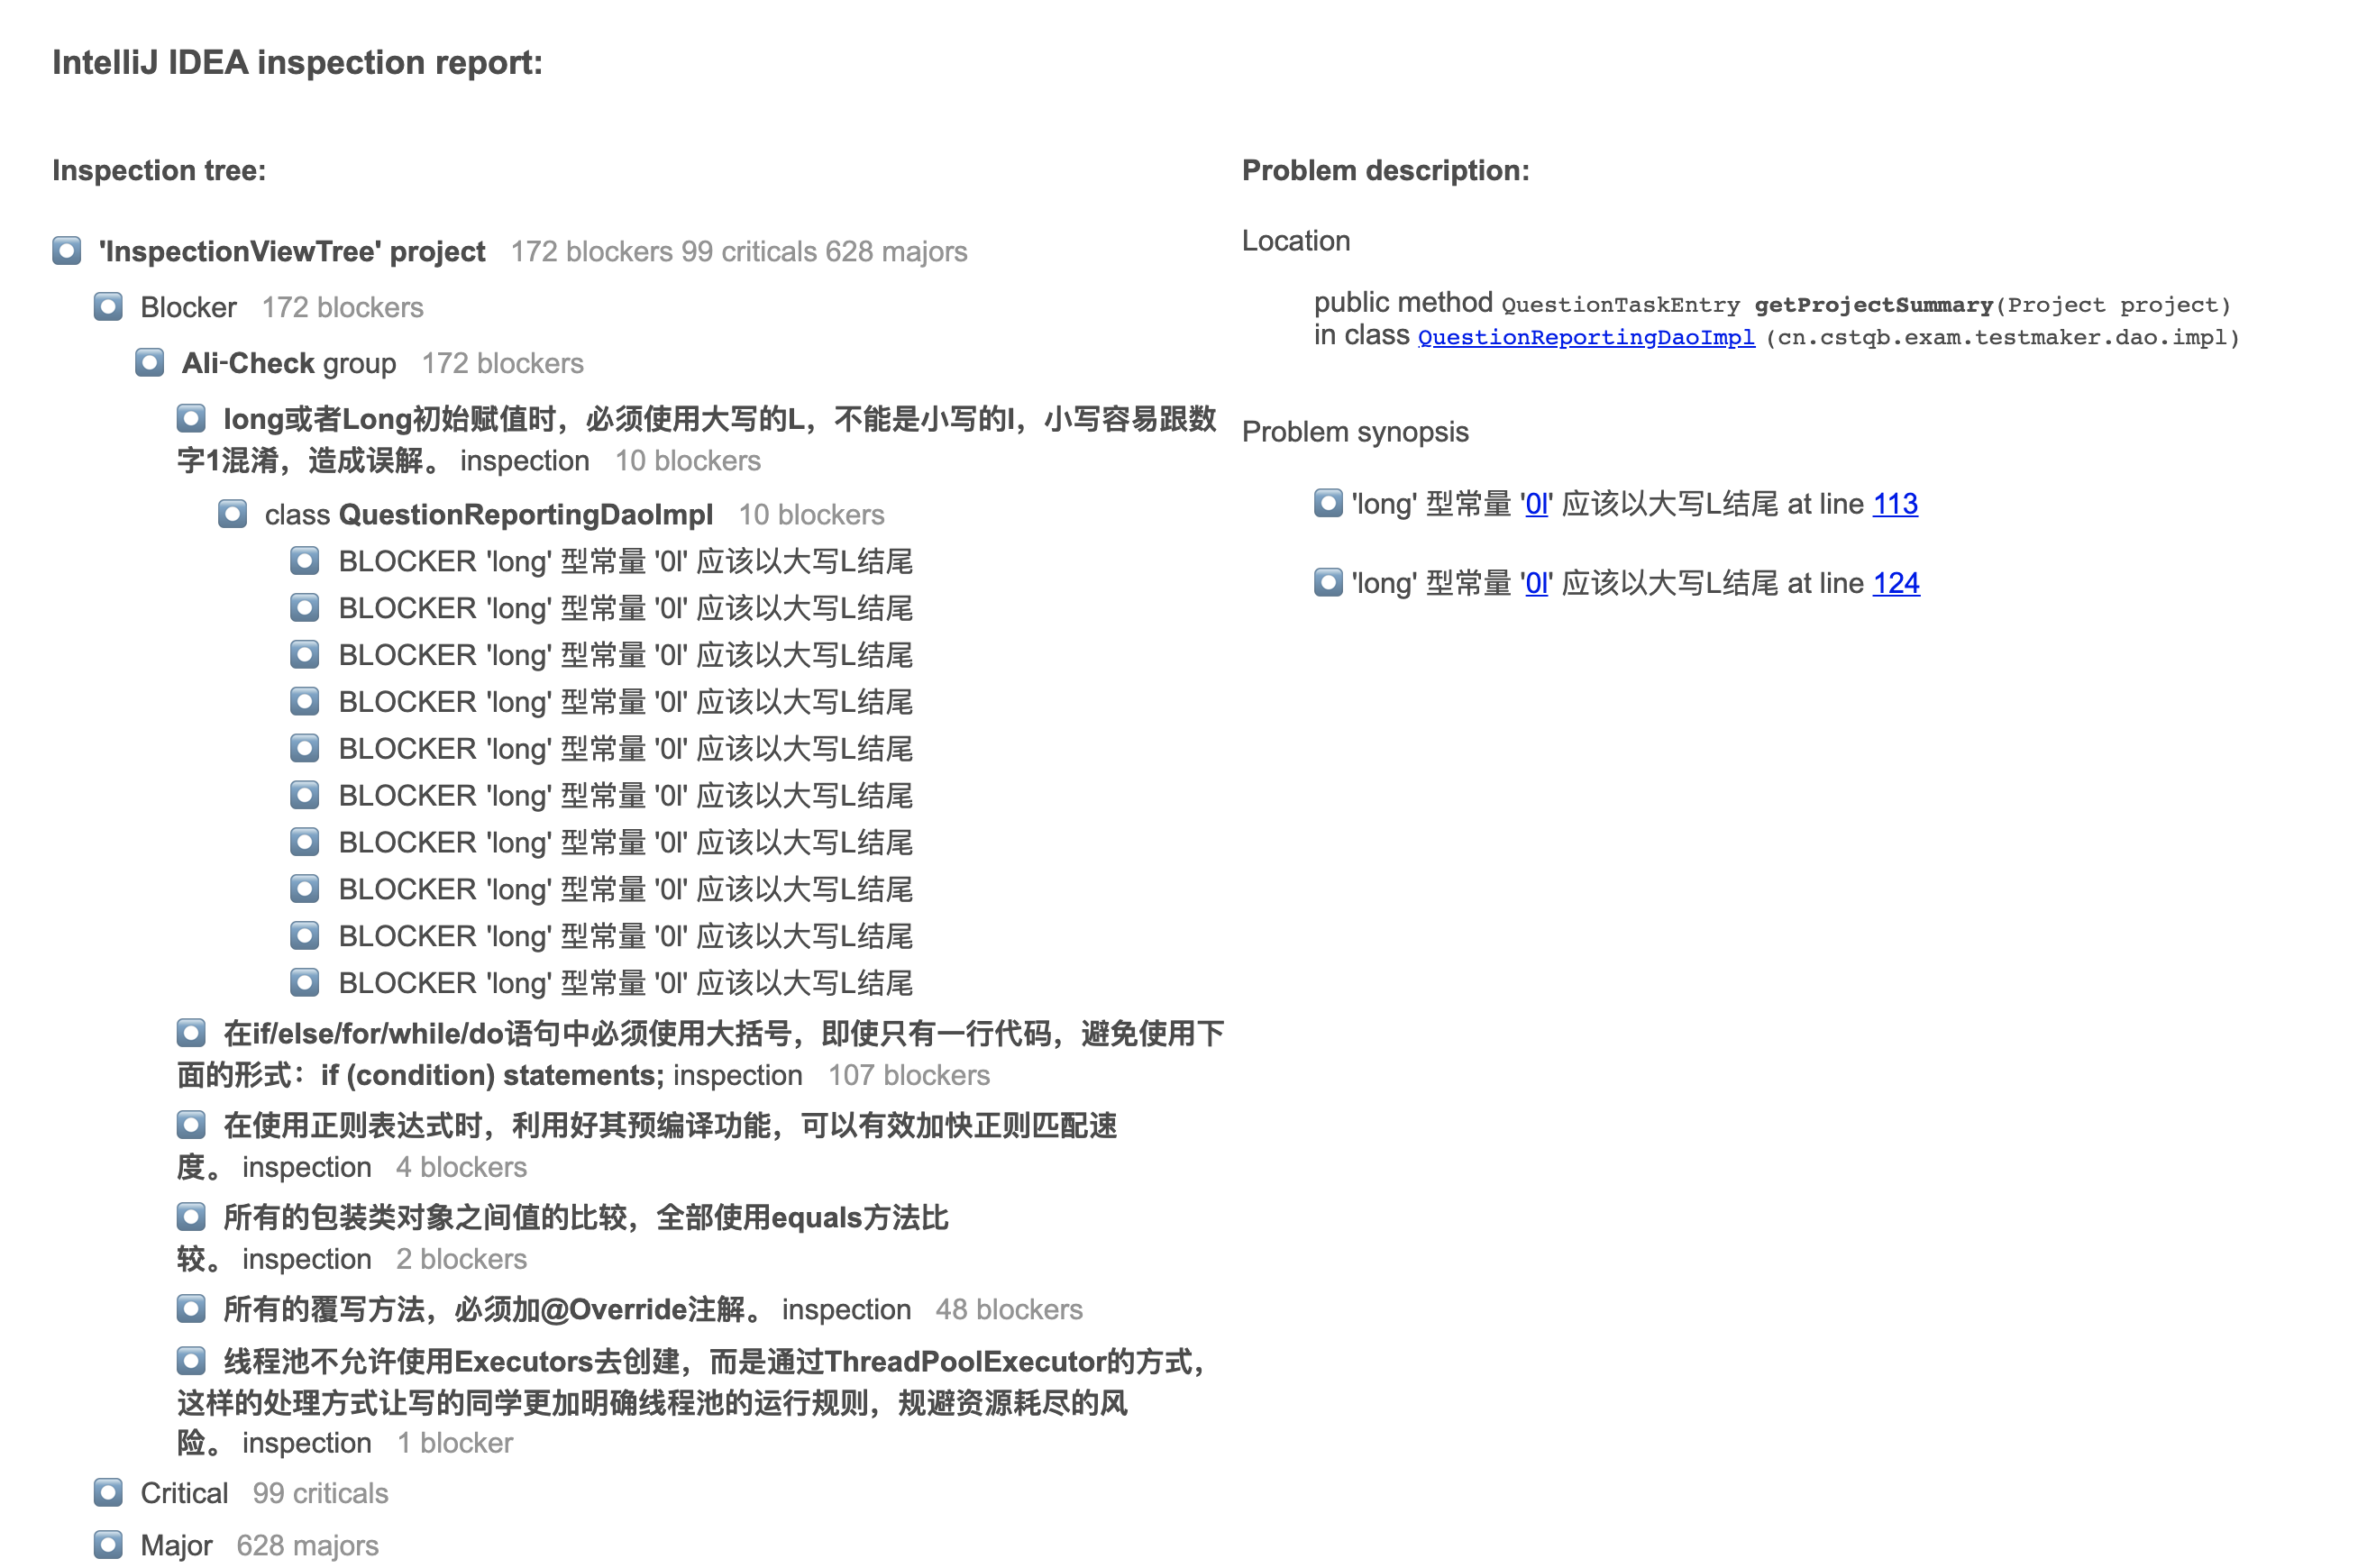
\includegraphics{screenshots/pic1.jpg}
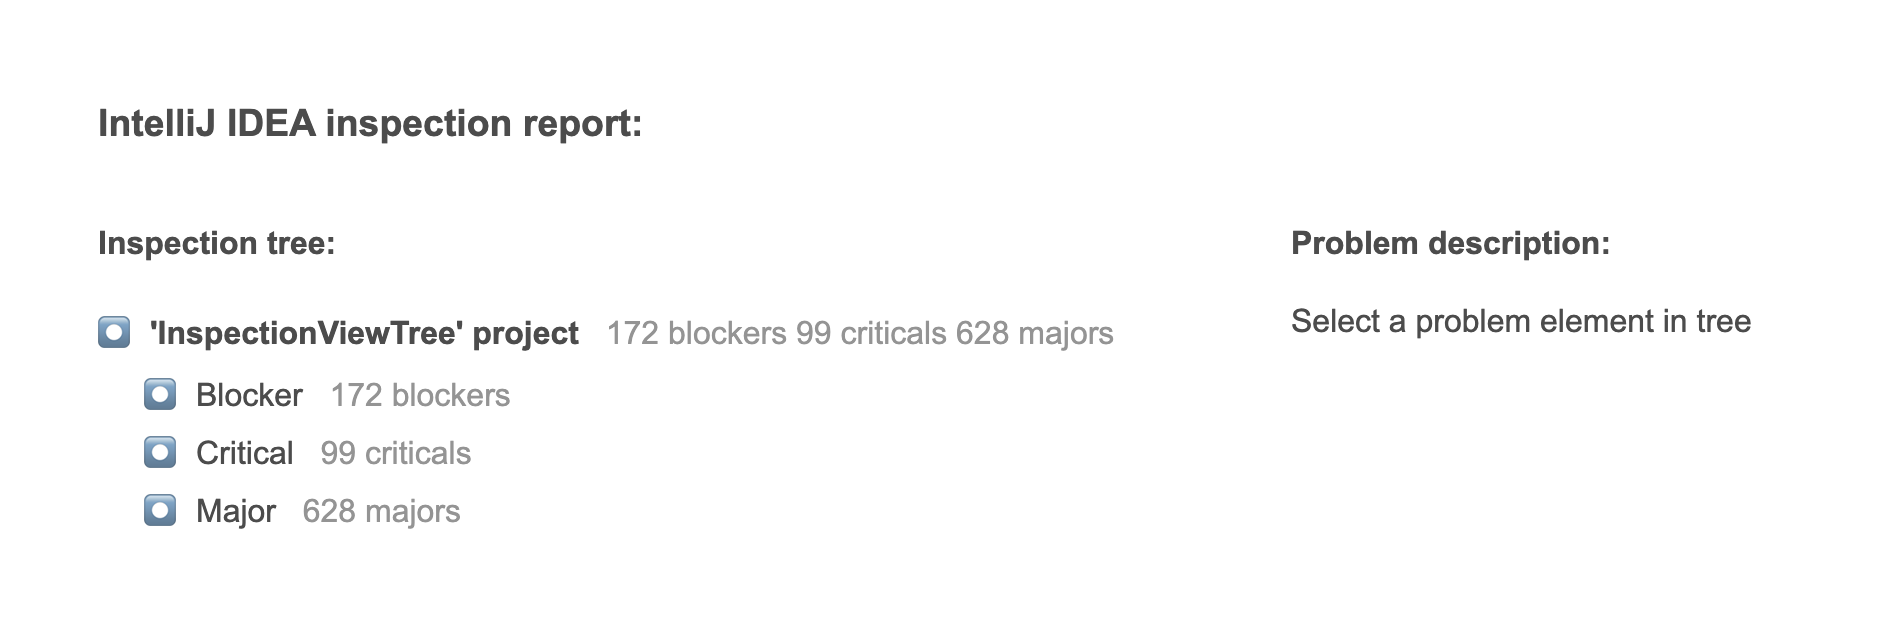
\includegraphics{screenshots/pic2.jpg}

\hypertarget{ux6d4bux8bd5ux7ed3ux679cux5206ux6790-1}{%
\subsection{测试结果分析}\label{ux6d4bux8bd5ux7ed3ux679cux5206ux6790-1}}

\hypertarget{ux4e0dux540cux5de5ux5177ux4e4bux95f4ux7684ux5bf9ux6bd4ux5206ux6790}{%
\section{不同工具之间的对比分析}\label{ux4e0dux540cux5de5ux5177ux4e4bux95f4ux7684ux5bf9ux6bd4ux5206ux6790}}

\hypertarget{ux6d4bux8bd5ux603bux7ed3}{%
\section{测试总结}\label{ux6d4bux8bd5ux603bux7ed3}}

\pagebreak

\hypertarget{ux53c2ux8003ux6587ux732e}{%
\section*{参考文献}\label{ux53c2ux8003ux6587ux732e}}
\addcontentsline{toc}{section}{参考文献}

\hypertarget{refs}{}
\leavevmode\hypertarget{ref-innovativeInternationalisation}{}%
International Organization for Standardization. 2014. \emph{Systems and
Software Engineering --- Systems and Software Quality Requirements and
Evaluation (SQuaRE) --- Guide to SQuaRE}. \emph{International
Organization for Standardization}. Vol. 2014.
\url{https://www.iso.org/standard/64764.html}.

\leavevmode\hypertarget{ref-innovative1}{}%
中国国家标准化管理委员会. 2016. \emph{GB/T
25000.51-2016《系统与软件工程系统与软件质量要求和评价 (SQuaRE) 第 51
部分 : 就绪可用软件产品 (RUSP) 的质量要求和测试细则》}.
\emph{系统与软件工程系统与软件质量要求和评价 (SQuaRE)}. Vol. 51.
中国国家标准化管理委员会. \url{http://openstd.samr.gov.cn}.

\leavevmode\hypertarget{ref-innovative3}{}%
---------. 2017a. \emph{GB/T 25000.12-2017《系统与软件工程
系统与软件质量要求和评价(SQuaRE) 第12部分:数据质量模型》}.
\emph{系统与软件工程系统与软件质量要求和评价 (SQuaRE)}. Vol. 12.
中国国家标准化管理委员会. \url{http://openstd.samr.gov.cn}.

\leavevmode\hypertarget{ref-innovative4}{}%
---------. 2017b. \emph{GB/T 25000.24-2017《系统与软件工程
系统与软件质量要求和评价(SQuaRE) 第24部分:数据质量测量》}.
\emph{系统与软件工程系统与软件质量要求和评价 (SQuaRE)}. Vol. 24.
中国国家标准化管理委员会. \url{http://openstd.samr.gov.cn}.

\leavevmode\hypertarget{ref-innovative5}{}%
---------. 2018. \emph{GB/T 25000.40-201《系统与软件工程
系统与软件质量要求和评价(SQuaRE) 第40部分:评价过程》}.
\emph{系统与软件工程系统与软件质量要求和评价 (SQuaRE)}. Vol. 40.
中国国家标准化管理委员会. \url{http://openstd.samr.gov.cn}.

\leavevmode\hypertarget{ref-innovative2}{}%
---------. 2019. \emph{GB/T 25000.23-2019《系统与软件工程
系统与软件质量要求和评价(SQuaRE) 第23部分:系统与软件产品质量测量》}.
\emph{系统与软件工程系统与软件质量要求和评价 (SQuaRE)}. Vol. 23.
中国国家标准化管理委员会. \url{http://openstd.samr.gov.cn}.

\end{document}
